\documentclass[12pt,answers]{exam}


\usepackage[margin=0.8in,footskip=0.2in]{geometry}

\usepackage{etex}
\usepackage{amssymb,amsmath,multicol} %<-- InWorksheetExam1 i also have fancyhdr,

\usepackage[metapost]{mfpic}
\usepackage[pdftex]{graphicx}

\usepackage{pst-plot}
\usepackage{pgfplots}
\pgfplotsset{compat=1.9}

\usepackage{tikz}
\usepackage{tkz-2d}
\usepackage{tkz-base}
\usetikzlibrary{calc}

\usepackage{tabularx, booktabs}
\newcolumntype{Y}{>{\centering\arraybackslash}X}

\usepackage{array}
\newcolumntype{L}[1]{>{\raggedright\let\newline\\\arraybackslash\hspace{0pt}}m{#1}}
\newcolumntype{C}[1]{>{\centering\let\newline\\\arraybackslash\hspace{0pt}}m{#1}}
\newcolumntype{R}[1]{>{\raggedleft\let\newline\\\arraybackslash\hspace{0pt}}m{#1}}

\newcommand\T{\rule{0pt}{2.6ex}}       % Top strut
\newcommand\B{\rule[-1.2ex]{0pt}{0pt}} % Bottom strut

\usepackage[inline]{enumitem}
\usepackage{refcount}%<-- non in WorksheetExam1

\usepackage{pstricks-add,pst-eucl}
\usepackage{caption}

\def\f{x+1} \def\g{-x/3+2}  \def\h{-x+3}

\newcommand{\vasymptote}[2][]{
	\draw [densely dashed,#1] ({rel axis cs:0,0} -| {axis cs:#2,0}) -- ({rel axis cs:0,1} -| {axis cs:#2,0});
}

\newcommand*\circled[1]{\tikz[baseline=(char.base)]{%
		\node[shape=circle,draw,inner sep=1pt] (char) {#1};}}
\renewcommand\choicelabel{\circled{\thechoice}}


\let\originalleft\left
\let\originalright\right
\renewcommand{\left}{\mathopen{}\mathclose\bgroup\originalleft}
\renewcommand{\right}{\aftergroup\egroup\originalright}

\addpoints
%\printanswers
\noprintanswers

\usepackage{geometry}
\geometry{
	%a4paper,
	%total={170mm,257mm},
	%left=20mm,
	%top=20mm,
	text={.95\paperwidth,.95\paperheight}, ratio=1:3,%includefoot
}

\opengraphsfile{Q11a_Spring_16}

\begin{document}
%\extrawidth{-0.3in}
\pagestyle{headandfoot}

%\setlength{\hoffset}{-.25in}

%\extraheadheight{-.3in}
\runningheadrule
\firstpageheader{\bfseries {MATH1-UC 1171}}{ \bfseries {Quiz 11 }}{\bfseries {4/26/2016}} 



\firstpagefooter{} %%&&CHANGED
                {}
                {Points earned: \hbox to 0.5in{\hrulefill}
                 out of  \pointsonpage{\thepage} points}
                 
						

%\vspace*{0.1cm}
\hbox to \textwidth { \scshape {Name:} \enspace\hrulefill}
\vspace{0.1in}




\pointpoints{point}{points}

\begin{questions}


\addpoints

\question A Ferris wheel with 10 capsules has a diameter of 28 meters and its lowest point (at the 6 o'clock position) is 2 meters above the ground. One full rotation of the wheel takes 12 minutes, and the wheel rotates counterclockwise at a constant speed. The capsules are labeled from 1 to 10. We start observing when capsule 1 is at the highest point on the wheel. 
 Let $H(t)$ be the height of capsule 1 $t$ minutes after we start the observation. 

\begin{parts}
\part[2] Fill out this table:

\begin{minipage}{\linewidth}
\centering
%\captionof{table}{} %\label{tab:title} 
\begin{tabular}{|L{1.5cm}|C{0.8cm}|C{0.8cm}|C{0.8cm}|C{0.8cm}|C{0.8cm}|}
\hline
$t$         &0&3& 6 & 9 & 12  \T\B   \\ \hline
$H(t)$   & & &     &     &         \T\B             \\ \hline
\end{tabular}
\end{minipage}
\part[2] \label{part:partettob} On the grid provided below, draw the graph of $H(t)$ for $\displaystyle 0\leq t \leq 12$. Label the tick marks on the horizontal and vertical axes.
	
	
	
\begin{tikzpicture}
	\draw[gray!50, thin, step=0.5] (-7,-3) grid (7,3);
	\end{tikzpicture}
\part[1] The amplitude of the graph in part (\ref{part:partettob}) is: \hbox to 1in{\dotfill} \part[1] The period of the graph in part (\ref{part:partettob}) is: \hbox to 1in{\dotfill}
\part[1] The equation of the midline of the graph in part (\ref{part:partettob}) is: \hbox to 1in{\dotfill}
\end{parts}
\question Suppose that the terminal point determined by $t$ is $\displaystyle \left(\frac{3}{5},\frac{4}{5}\right )$. 
\begin{parts}
\part[2] Find the coordinates of the terminal point of $-t$\dotfill

\part[2] Find the coordinates of the terminal point of $2\pi + t$\dotfill


\bonuspart[2] Find the coordinates of the terminal point of $t- \pi $\dotfill
\end{parts}
\question[1] As a wave passes by an offshore piling, the height of the water is modeled by the function
$\displaystyle h(t) = 9 \cos\left (\frac{\pi}{10}t\right )$ where $h(t)$ is the height in feet above mean sea level at time $t$ seconds. Find the wave height, that is, the vertical distance between the trough and the crest of the wave.
%\fillwithdottedlines{1cm]
\fillwithdottedlines{2.5cm}


\end{questions}
 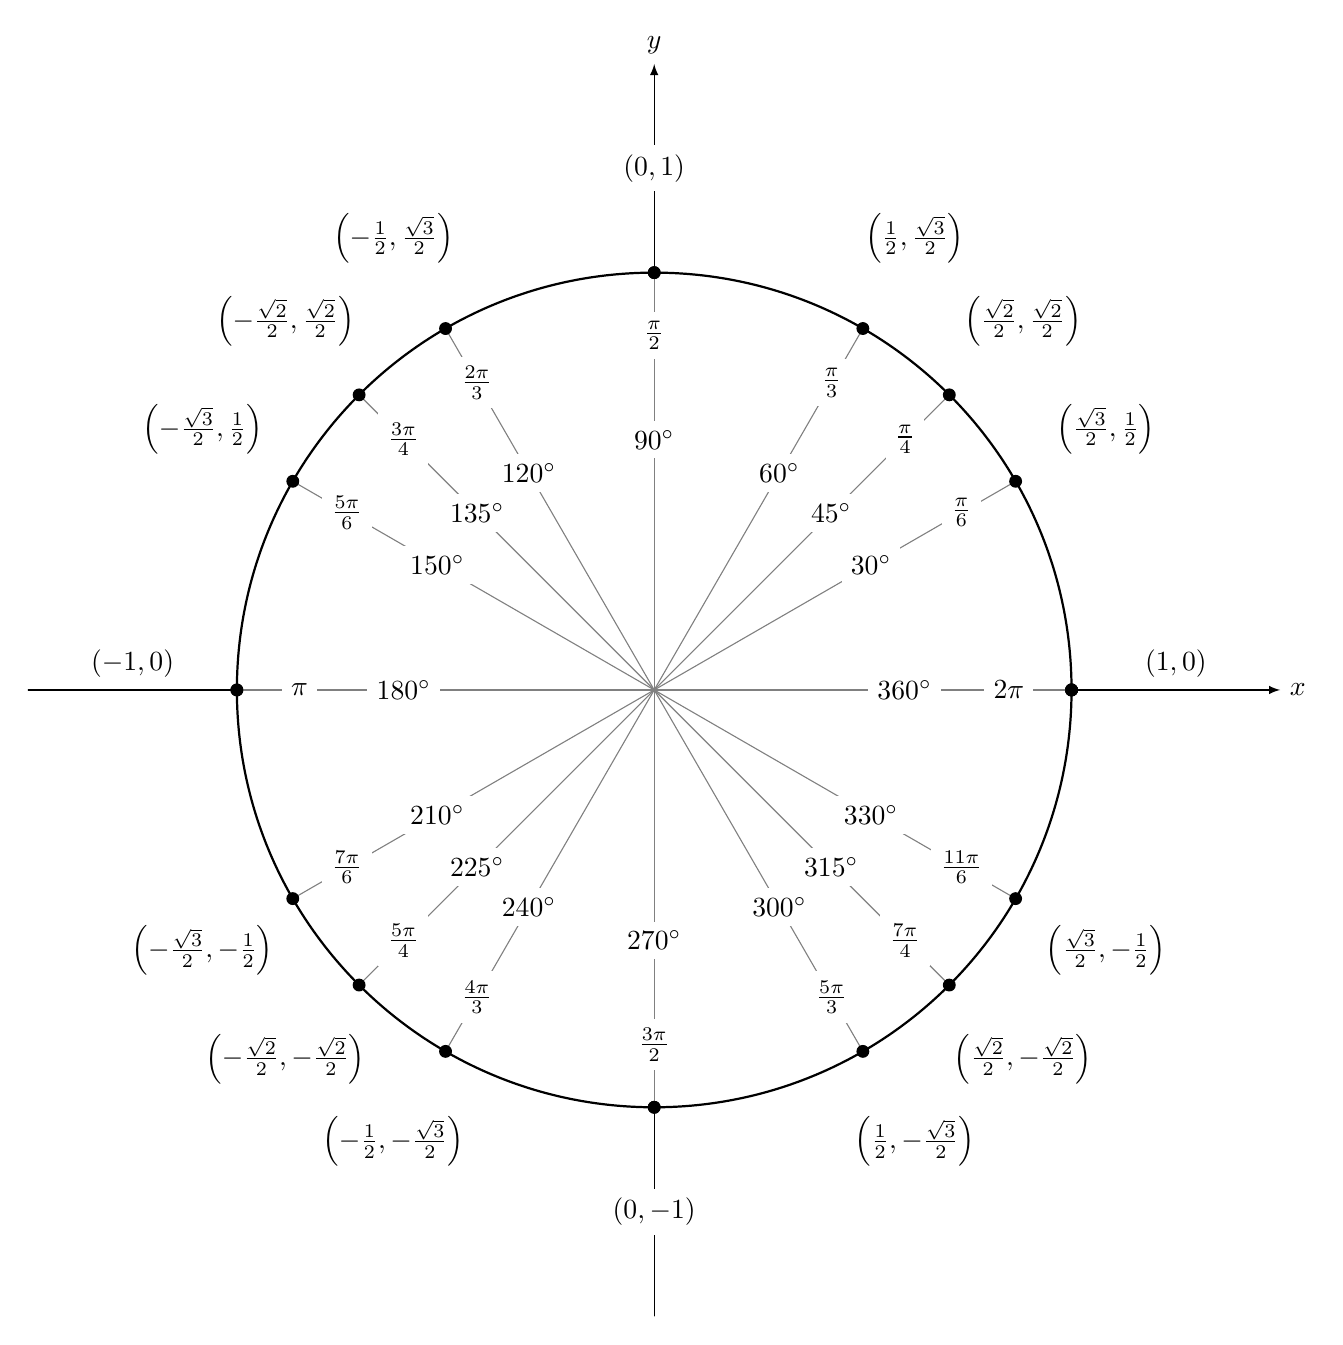
\begin{tikzpicture}[scale=5.3,cap=round,>=latex]
        % draw the coordinates
        \draw[->] (-1.5cm,0cm) -- (1.5cm,0cm) node[right,fill=white] {$x$};
        \draw[->] (0cm,-1.5cm) -- (0cm,1.5cm) node[above,fill=white] {$y$};

        % draw the unit circle
        \draw[thick] (0cm,0cm) circle(1cm);

        \foreach \x in {0,30,...,360} {
                % lines from center to point
                \draw[gray] (0cm,0cm) -- (\x:1cm);
                % dots at each point
                \filldraw[black] (\x:1cm) circle(0.4pt);
                % draw each angle in degrees
                \draw (\x:0.6cm) node[fill=white] {$\x^\circ$};
        }
        
        \foreach \x in {0,45,...,360} {
                % lines from center to point
                \draw[gray] (0cm,0cm) -- (\x:1cm);
                % dots at each point
                \filldraw[black] (\x:1cm) circle(0.4pt);
                % draw each angle in degrees
                \draw (\x:0.6cm) node[fill=white] {$\x^\circ$};
        }
        % draw each angle in radians
        \foreach \x/\xtext in {
            30/\frac{\pi}{6},
            45/\frac{\pi}{4},
            60/\frac{\pi}{3},
            90/\frac{\pi}{2},
            120/\frac{2\pi}{3},
            135/\frac{3\pi}{4},
            150/\frac{5\pi}{6},
            180/\pi,
            210/\frac{7\pi}{6},
            225/\frac{5\pi}{4},
            240/\frac{4\pi}{3},
            270/\frac{3\pi}{2},
            300/\frac{5\pi}{3},
            315/\frac{7\pi}{4},
            330/\frac{11\pi}{6},
            360/2\pi}
                \draw (\x:0.85cm) node[fill=white] {$\xtext$};

        \foreach \x/\xtext/\y in {
            % the coordinates for the first quadrant
            30/\frac{\sqrt{3}}{2}/\frac{1}{2},
            45/\frac{\sqrt{2}}{2}/\frac{\sqrt{2}}{2},
            60/\frac{1}{2}/\frac{\sqrt{3}}{2},
            % the coordinates for the second quadrant
            150/-\frac{\sqrt{3}}{2}/\frac{1}{2},
            135/-\frac{\sqrt{2}}{2}/\frac{\sqrt{2}}{2},
            120/-\frac{1}{2}/\frac{\sqrt{3}}{2},
            % the coordinates for the third quadrant
            210/-\frac{\sqrt{3}}{2}/-\frac{1}{2},
            225/-\frac{\sqrt{2}}{2}/-\frac{\sqrt{2}}{2},
            240/-\frac{1}{2}/-\frac{\sqrt{3}}{2},
            % the coordinates for the fourth quadrant
            330/\frac{\sqrt{3}}{2}/-\frac{1}{2},
            315/\frac{\sqrt{2}}{2}/-\frac{\sqrt{2}}{2},
            300/\frac{1}{2}/-\frac{\sqrt{3}}{2}}
                \draw (\x:1.25cm) node[fill=white] {$\left(\xtext,\y\right)$};

        % draw the horizontal and vertical coordinates
        % the placement is better this way
        \draw (-1.25cm,0cm) node[above=1pt] {$(-1,0)$}
              (1.25cm,0cm)  node[above=1pt] {$(1,0)$}
              (0cm,-1.25cm) node[fill=white] {$(0,-1)$}
              (0cm,1.25cm)  node[fill=white] {$(0,1)$};
    \end{tikzpicture}
\end{document}                 